\subsection{IBM BladeCenter S}

Para aceder ao bladecenter S, existe instalado um (ou mais) AMM (Advanced Managment Module). O mesmo deverá ser acedido via web em http://ip\_do\_bladecenter/

\begin{figure}[H]
    \begin{center}
        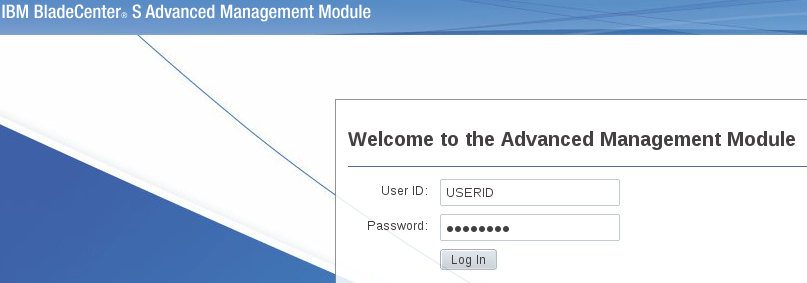
\includegraphics[width=10cm]{include/img/amm_bladecenterS_1}
    \end{center}
    \caption{Ecrã inicial do AMM}
    \label{fig:amm-1}
\end{figure}

As credenciais por omissão são:
\begin{itemize}
\item Username: USERID
\item Password: PASSW0RD   (com zero em vez de O)
\end{itemize}

No entanto as credenciais podem ter sido alteradas. Por favor consulte as informações fornecidas caso as credenciais não sejam estas.

Depois deve carregar com o botão "Log In" e deve aparecer um ecrã como o seguinte indicando o timeout da ligação:

\begin{figure}[H]
    \begin{center}
        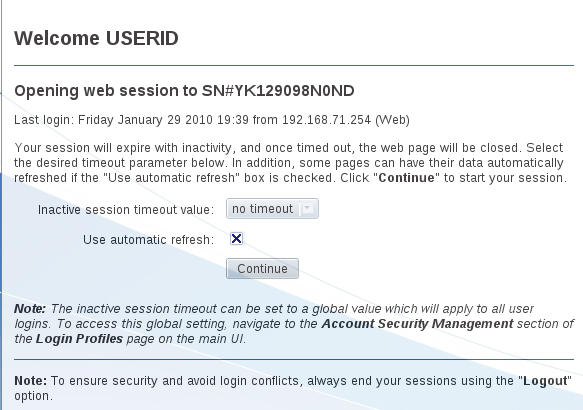
\includegraphics[width=10cm]{include/img/amm_bladecenterS_2}
    \end{center}
    \caption{Timeout de ligação}
    \label{fig:amm-2}
\end{figure}

Deverá carregar no botão "Continue" e deverá aparecer uma página semelhante à seguinte:

\begin{figure}[H]
    \begin{center}
        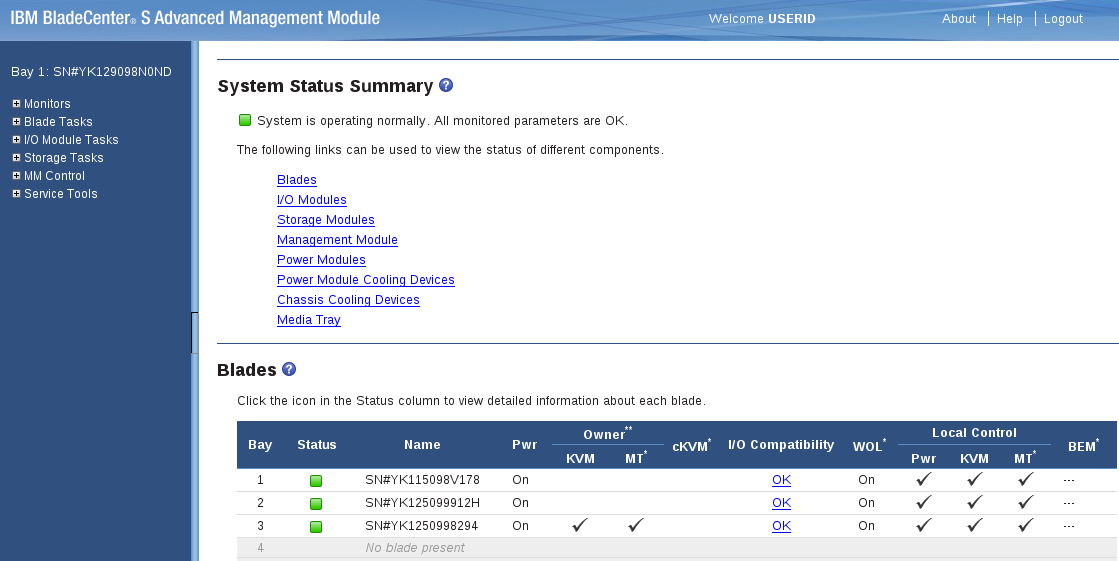
\includegraphics[width=10cm]{include/img/amm_bladecenterS_3}
    \end{center}
    \caption{Ecrã principal do AMM}
    \label{fig:amm-3}
\end{figure}


Posteriormente poderá efectuar a gestão do bladecenter. Para mais informação consulte o manual do bladecenter na página da IBM em \url{ftp://ftp.software.ibm.com/systems/support/system\_x\_pdf/44r5274.pdf}.

No caso de lhe ser solicitado pelo suporde da IBM poderá encontrar toda a informação relativa ao bladecenter em "Service Tools"->"AMM Service Data", tal como pode ver pela imagem seguinte:

\begin{figure}[H]
    \begin{center}
        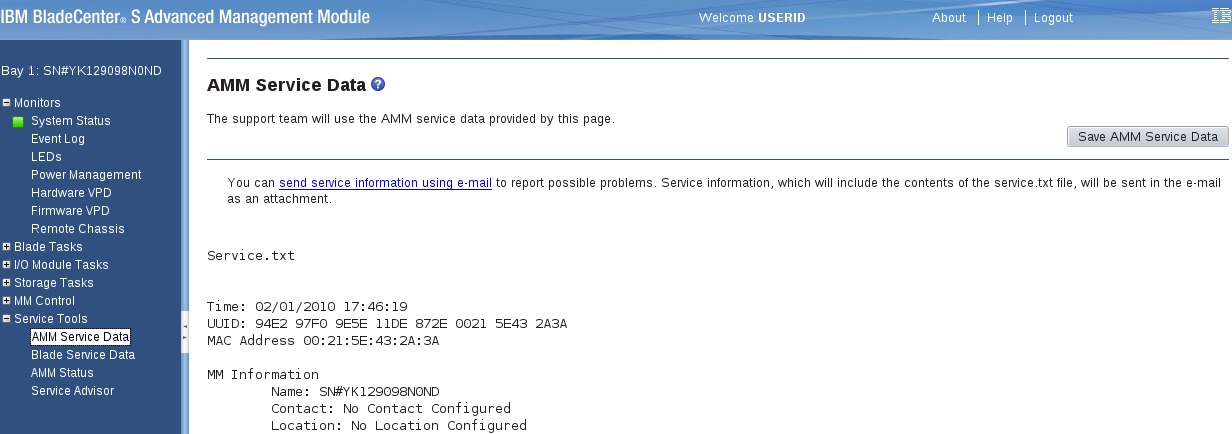
\includegraphics[width=10cm]{include/img/amm_bladecenterS_4}
    \end{center}
    \caption{Ecrã Service Data}
    \label{fig:amm-4}
\end{figure}


